\documentclass[11pt,letterpaper]{article}
\usepackage[T1]{fontenc}
\usepackage[utf8]{inputenc}
\usepackage{amsmath,amsthm}
\usepackage{newtxtext,newtxmath}
\usepackage[margin=0.93in,headheight=14pt]{geometry}
\usepackage{microtype}
\usepackage[table]{xcolor}
\usepackage{booktabs,array,longtable,tabularx}
\usepackage{enumitem}
\usepackage{tikz}
\usetikzlibrary{positioning,calc,arrows.meta}
\usepackage[most]{tcolorbox}
\usepackage{fancyhdr}
\usepackage{listings}
\usepackage{xurl}
\usepackage[colorlinks=true]{hyperref}
\usepackage[nameinlink,noabbrev]{cleveref}
\definecolor{Olive}{HTML}{596348}
\definecolor{PaleOlive}{HTML}{F1F2EA}
\definecolor{Ink}{HTML}{29312B}
\definecolor{Muted}{HTML}{626A61}
\hypersetup{linkcolor=Olive,citecolor=Olive,urlcolor=Olive,
 pdftitle={A counterexample to winner stability in ordinal Chomp},
 pdfsubject={A certified proof that ch(4,6,9)=2},
 pdfauthor={Research report prepared for Vladimir Reshetnikov}}
\pagestyle{fancy}
\fancyhf{}
\fancyhead[L]{\small\itshape A counterexample in ordinal Chomp}
\fancyhead[R]{\small September 2026}
\fancyfoot[C]{\small\thepage}
\renewcommand{\headrulewidth}{0.3pt}
\setlength{\parskip}{3pt}
\setlength{\parindent}{1.2em}
\setlength{\emergencystretch}{2em}
\setlist{itemsep=2pt,topsep=4pt}
\numberwithin{equation}{section}
\newtheorem{theorem}{Theorem}[section]
\newtheorem{lemma}[theorem]{Lemma}
\newtheorem{proposition}[theorem]{Proposition}
\newtheorem{corollary}[theorem]{Corollary}
\theoremstyle{definition}
\newtheorem{definition}[theorem]{Definition}
\newtheorem{example}[theorem]{Example}
\newtheorem{remark}[theorem]{Remark}
\newcommand{\N}{\mathbb N}
\newcommand{\Ord}{\mathrm{Ord}}
\newcommand{\Sg}{\mathcal S}
\newcommand{\Gr}{\operatorname{g}}
\newcommand{\Ap}{\operatorname{Ap}}
\newcommand{\mex}{\operatorname{mex}}
\newcommand{\ex}{\operatorname{ex}}
\newcommand{\ch}{\operatorname{ch}}
\newcommand{\Opt}{\mathcal O}
\newcommand{\ps}{\mathbin{\boxplus}}
\newcommand{\xo}{\mathbin{\oplus_{\!2}}}
\renewcommand{\Game}{\mathsf G}
\newcommand{\Poison}{\mathsf H}
\newcommand{\DiamondGame}{\mathsf D}
\newcommand{\KGame}{\mathsf K}
\newcommand{\RGame}{\mathsf R}
\newcommand{\smallmex}{\operatorname{mex}_{2}}
\newtcolorbox{resultbox}{enhanced,breakable,colback=PaleOlive,colframe=Olive,
 boxrule=0.6pt,arc=1mm,left=10pt,right=10pt,top=8pt,bottom=8pt}
\lstset{language=Python,basicstyle=\ttfamily\footnotesize,
 keywordstyle=\color{Olive}\bfseries,commentstyle=\color{Muted}\itshape,
 stringstyle=\color{Olive},showstringspaces=false,breaklines=true,
 frame=single,rulecolor=\color{Olive!40},xleftmargin=4pt,xrightmargin=4pt,
 columns=fullflexible,keepspaces=true,tabsize=4}

\title{\vspace{-1.2em}\color{Ink}\bfseries
 A counterexample to winner stability\\[3pt] in ordinal Chomp}
\author{Research report prepared for Vladimir Reshetnikov}
\date{19 September 2026}

\begin{document}
\maketitle
\thispagestyle{empty}
\begin{abstract}
Let $\Sg=\langle4,6,9\rangle$ be the numerical semigroup ordered by
$x\leq_{\Sg}y$ when $y-x\in\Sg$. We give a computer-assisted proof that
Chomp on $\Sg$ is a second-player win, whereas Chomp on its ordinal square
$\Sg^2=\{\omega a+b:a,b\in\Sg\}$ is a first-player win. An explicit winning
first move is $\omega\cdot4+4$. The same move wins on every higher ordinal
extension, so $\ch(4,6,9)=2$. This contradicts the winner-stability conjecture
in the first version of Rivero Herrera's paper and answers its current
Question~4.6 negatively already for finite natural-number generators.

The infinite-game calculation needs only the first four entries of an
option-value spectrum. Its one additional numerical ingredient is that
$\Gr(\Ap(\Sg,t)\setminus\{0\})\neq1$ for every positive $t\in\Sg$.
We certify the stronger inequality $\Gr(\Ap(\Sg,t)\setminus\{0\})\geq2$
by a deterministic recurrence on 17 gap ideals. Its bounded-Grundy boundary
state repeats after 28 steps. Every entry of the finite certificate is also
verified by a separate, untruncated finite-poset computation. A general
bounded-Grundy eventual-periodicity theorem explains why the certificate
proves a universal statement, rather than merely supporting one numerically.
\end{abstract}

\begin{resultbox}
\textbf{Main conclusion.}
\[
\boxed{\quad\ch(4,6,9)=2,\qquad
 \text{winning first move }\omega\cdot4+4.\quad}
\]
The proof below includes an exact finite certificate, not an assumed
stabilization of a numerical search. The two implementations supplied with
this report were executed successfully. The result has not been externally
refereed or formalized in a proof assistant.
\end{resultbox}

\vspace{3pt}
\noindent\textbf{Keywords.} Poset games; numerical semigroups; ordinal powers;
Ap\'ery sets; Sprague--Grundy theory; finite-state certificates.

\clearpage
\tableofcontents
\clearpage

\section{The question and the result}
\label{sec:question}

Numerical-semigroup Chomp provides a particularly concrete meeting point of
order theory, infinite games, and ordinal arithmetic. A semigroup gives an
infinite, locally finite partial order on a subset of the natural numbers.
Replacing its elements by lexicographically arranged copies of the same
order produces ordinal extensions in which the options can themselves remain
infinite. The question is whether that extra order structure can change the
winner.

Rivero Herrera's April 2025 formulation asks whether a second-player win on
the first extension necessarily remains a second-player win on all ordinal
extensions \cite[Conjecture~4.1]{RiveroV1}. The January 2026 revision asks
whether the first winning exponent $\ch(\Gamma)$, when it exists, must have
its smallest possible value \cite[Question~4.6]{RiveroV3}. For a finite set
$\Gamma$ of positive natural numbers, that smallest value is $1$.
The latter question is credited in that revision to Ignacio Garc\'ia-Marco.

\begin{theorem}[Main result]\label{thm:main}
Put $\Sg=\langle4,6,9\rangle$. With the ordinal-extension order defined in
\cref{sec:objects}, the following hold.
\begin{enumerate}[label=\textup{(\roman*)}]
\item Chomp on $\Sg^1=\Sg$ is a second-player win.
\item Chomp on $\Sg^2$ is a first-player win. The move
      $\alpha=\omega\cdot4+4$ leaves a position of Grundy value $0$.
\item The same move wins on $\Sg^\sigma$ for every ordinal $\sigma\geq2$.
      Consequently $\ch(4,6,9)=2$.
\end{enumerate}
\end{theorem}

The first assertion has an elementary proof using the symmetry of this
semigroup. The second is the substantive new calculation. It uses a finite
certificate for a low-value exclusion, not a simulation of an infinite
board. The third follows because the chosen move removes every newly added
higher-order block.

\subsection{What is being claimed}

The assertion is a counterexample within the numerical-semigroup family,
not merely within arbitrary pointed partially ordered sets. Winner changes
for arbitrary finite pointed posets are already exhibited in
\cite[Example~3.2]{RiveroV3}; those examples do not answer the semigroup
question. Conversely, this counterexample does not contradict any asserted
countable upper bound for a transition exponent: it realizes the very small
nontrivial value $2$.

The source check for this report found the question still present in the
latest arXiv version, dated 5 January 2026, and found no later resolution.
That is a statement about the literature located in this investigation,
not a claim to have exhaustively searched unpublished work. The mathematical
claim is supported by the complete reduction and executable certificate
below, independently of its eventual priority assessment.

\subsection{Proof architecture}

The proof has three logically separate parts. First, an elementary
calculation gives the semigroup's gaps and an Ap\'ery diamond. Second,
Sprague--Grundy algebra turns one excluded option value into a winning move
in the square. Third, a finite-state calculation establishes that exclusion
for every possible first move in the base semigroup.

The infinite conclusion is not obtained by replacing a sufficiently large
finite board by an infinite one. No such approximation is used. The only
limit argument is the induction that follows an exactly repeated state of
a deterministic recurrence.

\section{Orders, ordinal extensions, and game conventions}
\label{sec:objects}

\subsection{Numerical-semigroup orders}

Throughout, $\N=\{0,1,2,\ldots\}$. A numerical semigroup is an additive
submonoid $\Sg\subseteq\N$ with finite complement. Its natural semigroup
order is
\begin{equation}\label{eq:semigroup-order}
 x\leq_{\Sg}y\quad\Longleftrightarrow\quad y-x\in\Sg.
\end{equation}
Here a negative integer is not an element of $\Sg$. In particular, $0$ is the
least element, and $x\leq_{\Sg}y$ implies $x\leq y$ in the ordinary order.
The order need not be linear: in our example, $6$ and $9$ are incomparable
because $9-6=3\notin\Sg$.

For positive $t\in\Sg$, define
\begin{equation}\label{eq:apery}
 \Ap(\Sg,t)=\Sg\setminus(t+\Sg).
\end{equation}
This is exactly the surviving board after selecting $t$. If $F$ is the
largest gap of $\Sg$, every member of $\Ap(\Sg,t)$ is at most $t+F$, so the
board is finite. We write $\Ap(\Sg,0)=\varnothing$ when discussing the
ordinary, unpoisoned game.

The study of this game, including the symmetric-semigroup second-player
result and the finite-boundary representation used later, originates in
Garc\'ia-Marco and Knauer \cite{GMK}. We prove the particular facts needed
here rather than treating their general theorems as black boxes.

\subsection{The ordinal extension and its lexicographic description}

For an ordinal $\sigma$, let $\Sg^\sigma$ consist of $0$ and the ordinals
whose Cantor normal forms are
\begin{equation}\label{eq:cnf}
 \omega^{\beta_0}s_0+\cdots+\omega^{\beta_{r-1}}s_{r-1},
 \qquad \sigma>\beta_0>\cdots>\beta_{r-1},\qquad
 s_i\in\Sg\setminus\{0\}.
\end{equation}
Thus $\Sg^0=\{0\}$ and
\[
 \Sg^1=\Sg,\qquad
 \Sg^2=\{\omega a+b:a,b\in\Sg\}.
\]
For finite natural-number generators this is the coefficientwise description
of the naturally generated ordinal submonoids used in
\cite{RiveroV1,RiveroV3}.

The partial order is defined using \emph{ordinary ordinal subtraction}:
\begin{equation}\label{eq:ordinal-order}
 \alpha\leq_{\Sg^\sigma}\beta
 \quad\Longleftrightarrow\quad
 \alpha\leq\beta\ \text{and}\ \beta-\alpha\in\Sg^\sigma,
\end{equation}
where $\beta-\alpha$ is the unique $\gamma$ with $\alpha+\gamma=\beta$.
It is not coefficientwise subtraction under the natural sum.

For the square, \cref{eq:ordinal-order} becomes the strict lexicographic
rule
\begin{equation}\label{eq:lex}
 (a,b)\leq(c,d)
 \quad\Longleftrightarrow\quad
 a<_{\Sg}c\ \text{or}\ (a=c\ \text{and}\ b\leq_{\Sg}d),
\end{equation}
under the identification $(a,b)\leftrightarrow\omega a+b$.
Indeed, if $a<c$ then
\[
 (\omega c+d)-(\omega a+b)=\omega(c-a)+d;
\]
if $a=c$ and $b\leq d$, the difference is $d-b$. This also explains why
we must write $\omega\cdot4+4$, not $4\cdot\omega+4$: these are different
ordinals.

\subsection{Poisoned and unpoisoned games}

For a poset with minimum $0$, Chomp makes $0$ a poisoned move. Equivalently,
we delete $0$ in advance and play the normal poset game: a move removes its
chosen element and every greater element; a player with no legal move loses.
This convention makes the game an ordinary impartial normal-play game.

We distinguish two games on the same semigroup:
\[
 \Game=\text{the normal poset game on all of }\Sg,
 \qquad
 \Poison=\text{the normal poset game on }\Sg\setminus\{0\}.
\]
Thus $\Poison$ is semigroup Chomp, while $\Game$ has a legal move at $0$.
For a finite surviving board $D$ containing $0$, its poisoned version is
$D\setminus\{0\}$ and its unpoisoned version is $D$ itself.

Every play of either game on $\Sg$ terminates: its first move either empties
the board or leaves a finite Ap\'ery set. After our prescribed move in the
square, only finitely many such blocks remain. Once a block is touched it
becomes finite, so every continuation also terminates. Thus all the Grundy
values used in the main argument are well defined, even though some games
have infinitely many options.

\section{The game algebra that detects the transition}
\label{sec:algebra}

For a terminating impartial game $X$, let
\[
 \Opt(X)=\{\Gr(X'):X\longrightarrow X'\},\qquad
 \Gr(X)=\mex\Opt(X).
\]
The mex is taken among ordinals if necessary. A position is a second-player
win precisely when its Grundy value is $0$. All option values of $\Game$
are finite, because each of its options is a finite poset.

Write $X\ps Y$ for the disjunctive sum. For finite Grundy values,
\[
 \Gr(X\ps Y)=\Gr(X)\xo\Gr(Y),
\]
where $\xo$ denotes binary xor, not Hessenberg's natural sum of ordinals.
In the \emph{ordinal sum of games} $X:Y$, a move in $X$ discards $Y$, whereas
a move in $Y$ leaves $X$ untouched. In poset terms, every element of the
lower game $X$ lies below every element of the upper game $Y$.

\begin{lemma}[Excluded-ordinal formula]\label{lem:ordinal-sum}
For a set $A$ of ordinals, let $\ex_\eta(A)$ be the $\eta$-th ordinal not
in $A$, counting from $0$. Then
\begin{equation}\label{eq:ordinal-sum}
 \Gr(X:Y)=\ex_{\Gr(Y)}\bigl(\Opt(X)\bigr).
\end{equation}
In particular, if $\Gr(X)=\Gr(Y)=0$, then $\Gr(X:Y)=0$.
\end{lemma}

\begin{proof}
This is the ordinal-sum formula recorded in
\cite[Theorem~2.6]{GT}; the short proof fixes the convention.
Put $A=\Opt(X)$ and induct on the game tree of $Y$. Moves in $X$ supply
exactly the values in $A$. By induction, moves in $Y$ supply
$\ex_b(A)$ for $b\in\Opt(Y)$. Every ordinal outside $A$ occurs uniquely
as some $\ex_b(A)$, and these ordinals increase with $b$. The first index
missing from $\Opt(Y)$ is $\Gr(Y)$, so the mex of the combined option set
is $\ex_{\Gr(Y)}(A)$. The final assertion uses
$\ex_0(A)=\mex A=\Gr(X)$.
\end{proof}

\begin{corollary}[Adding a legal minimum]\label{cor:min-shift}
If $D$ is a finite poset with least element $0$, then
\begin{equation}\label{eq:min-shift}
 \Gr(D)=1+\Gr(D\setminus\{0\}).
\end{equation}
\end{corollary}
\begin{proof}
Write $D=\mathbf1:(D\setminus\{0\})$. Since
$\Opt(\mathbf1)=\{0\}$, the $n$-th excluded ordinal is $n+1$ for finite $n$.
\end{proof}

\subsection{A three-block detector}

\begin{lemma}[The low-value detector]\label{lem:detector}
Suppose $\Gr(\Game)=1$, all values in $B=\Opt(\Game)$ are finite, and
\begin{equation}\label{eq:low-spectrum}
 B\cap\{0,1,2,3\}=\{0,3\}.
\end{equation}
Then
\begin{equation}\label{eq:detector}
 \Gr\bigl((\Game\ps\Game):\Game\bigr)=3.
\end{equation}
\end{lemma}

\begin{proof}
For $L=\Game\ps\Game$, we have $\Gr(L)=1\xo1=0$ and
\[
 C:=\Opt(L)=\{b\xo1:b\in B\}.
\]
The assumed spectrum gives
\[
 1,2\in C,\qquad 0,3\notin C.
\]
Indeed, these four assertions correspond respectively to
$0,3\in B$ and $1,2\notin B$. All further finite option values are irrelevant
to the first two excluded ordinals. Therefore
$\ex_0(C)=0$ and $\ex_1(C)=3$. Apply \cref{lem:ordinal-sum} with upper-game
value $\Gr(\Game)=1$.
\end{proof}

\begin{remark}[Why a single nimber is not enough]\label{rem:substitution}
Replacing \emph{every} occurrence of $\Game$ by a singleton would be wrong.
A singleton also has Grundy value $1$, but
\[
 \Gr\bigl((\mathbf1\ps\mathbf1):\mathbf1\bigr)=2,
\]
not $3$. The lower components contribute their option spectrum, not just
their mex. The distinction is systematic in the ordered-join substitution
theory of \cite{GT}. In this proof the upper component can be summarized by
its Grundy value; the lower components cannot.
\end{remark}

\section{The semigroup and the winning first move}
\label{sec:counterexample}

\subsection{Gaps, symmetry, and the base game}

\begin{lemma}\label{lem:gaps}
For $\Sg=\langle4,6,9\rangle$,
\begin{equation}\label{eq:gaps}
 \N\setminus\Sg=\{1,2,3,5,7,11\}=:E.
\end{equation}
Its conductor is $12$, its largest gap is $F=11$, and for $0\leq n\leq11$,
\begin{equation}\label{eq:symmetry}
 n\in\Sg\quad\Longleftrightarrow\quad11-n\notin\Sg.
\end{equation}
\end{lemma}

\begin{proof}
Below $12$, the semigroup elements are exactly $0,4,6,8,9,10$.
Also $12=4+4+4$, $13=4+9$, $14=4+4+6$, and $15=6+9$.
Adding $4$ to these four consecutive elements gives every larger integer.
This proves \cref{eq:gaps}; the symmetry assertion is an inspection of the
six complementary pairs summing to $11$.
\end{proof}

\begin{lemma}\label{lem:base-losing}
For every positive $t\in\Sg$, $\Ap(\Sg,t)$ has a greatest element $t+11$.
Consequently
\begin{equation}\label{eq:base-values}
 \Gr(\Poison)=0,\qquad \Gr(\Game)=1.
\end{equation}
\end{lemma}

\begin{proof}
The integer $M=t+11$ lies in $\Sg$, but $M-t=11$ does not, so $M$ belongs
to the Ap\'ery set. Let $z$ be any other member. If $z<t$, then
$M-z>11$, hence $M-z\in\Sg$. If $z\geq t$, the difference $z-t$ is a gap,
and symmetry gives $M-z=11-(z-t)\in\Sg$. Thus $z\leq_{\Sg}M$.

A nonempty finite normal poset game with a greatest element cannot have
Grundy value $0$. Otherwise deleting the greatest element would leave a
winning position. A winning move from that position could have been played
directly in the original position, because it also deletes the greatest
element, a contradiction. Apply this argument to
$\Ap(\Sg,t)\setminus\{0\}$, whose greatest element is still $M$.
Every option of $\Poison$ is therefore nonzero, so $\Gr(\Poison)=0$.
Finally, the $0$ move in $\Game$ leaves the empty game, while each positive
move leaves a finite board of value at least $2$ by
\cref{cor:min-shift}. Its mex is $1$.
\end{proof}

This is a direct proof of the symmetric-semigroup phenomenon in this
particular case. It does \emph{not} establish the additional exclusion of
value $1$ from the poisoned Ap\'ery boards. That stronger fact is precisely
the finite-certificate lemma proved in \cref{sec:certificate}.

\subsection{The Ap\'ery diamond}

Since $4$ is the least positive semigroup element, it is an atom in the
semigroup order. Directly from \cref{eq:gaps},
\begin{equation}\label{eq:diamond}
 D:=\Ap(\Sg,4)=\{0,6,9,15\}.
\end{equation}
Its only strict cover relations are
$0<6<15$ and $0<9<15$. Let $\DiamondGame$ denote the unpoisoned normal game
on this four-point diamond. Its options have Grundy values
\begin{center}
\begin{tabular}{ccl}
\toprule
Move & Remaining value & Remaining shape\\
\midrule
$0$ & $0$ & Empty\\
$6$ & $2$ & The chain $0<9$\\
$9$ & $2$ & The chain $0<6$\\
$15$ & $1$ & A minimum below two incomparable points\\
\bottomrule
\end{tabular}
\end{center}
Hence
\begin{equation}\label{eq:diamond-value}
 \Gr(\DiamondGame)=3,
 \qquad \Gr(D\setminus\{0\})=2.
\end{equation}

\subsection{What remains after \texorpdfstring{$\omega\cdot4+4$}{omega*4+4}}

Select $(4,4)$ in the lexicographic square. The surviving outer coefficients
are $0,4,6,9,15$. At outer coefficient $4$, only the inner diamond $D$
remains. At $0,6,9,15$, the whole inner semigroup remains. Every other
outer coefficient is removed because it lies strictly above $4$ in the
semigroup order.

Among the surviving positive outer coefficients, $4$ is incomparable with
$6,9,15$: their positive differences from $4$ are respectively the gaps
$2,5,11$. Meanwhile $6$ and $9$ are incomparable and both lie below $15$.
The global poisoned point is $(0,0)$, so the outer-$0$ block is $\Poison$,
not $\Game$. Every element of that block lies below all other surviving
blocks. Thus the residual game is exactly
\begin{equation}\label{eq:residual}
 \RGame=\Poison:
 \left(\DiamondGame\ps\bigl((\Game\ps\Game):\Game\bigr)\right).
\end{equation}

\begin{figure}[htbp]
\centering
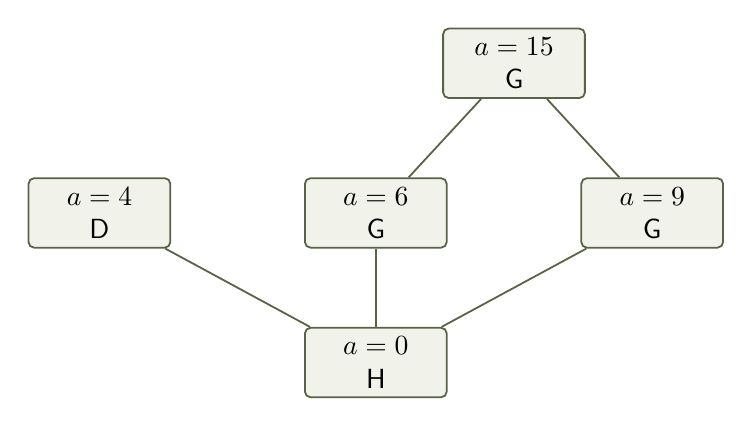
\begin{tikzpicture}[x=1.35cm,y=1.0cm,
 block/.style={draw=Olive,fill=PaleOlive,rounded corners=2pt,
 minimum width=1.8cm,minimum height=0.86cm,align=center},
 every path/.style={draw=Olive,line width=0.65pt}]
\node[block] (h) at (0,-0.3) {$a=0$\\$\Poison$};
\node[block] (d) at (-2.6,1.6) {$a=4$\\$\DiamondGame$};
\node[block] (g1) at (0,1.6) {$a=6$\\$\Game$};
\node[block] (g2) at (2.6,1.6) {$a=9$\\$\Game$};
\node[block] (g3) at (1.3,3.5) {$a=15$\\$\Game$};
\draw (h)--(d); \draw (h)--(g1); \draw (h)--(g2);
\draw (g1)--(g3); \draw (g2)--(g3);
\end{tikzpicture}
\caption{The exact residual block order. Each edge means that every element
of the lower block lies below every element of the upper block. The
poisoned point is removed only from the $a=0$ block.}
\label{fig:blocks}
\end{figure}

\begin{proof}[Proof of \cref{thm:main}, using the certified lemma]
The base-game statement is \cref{lem:base-losing}.
\Cref{lem:certified} below proves that each positive option of $\Game$
has value at least $3$. The zero move has value $0$, and the move $4$ has
value $3$ by \cref{eq:diamond-value}. Therefore
\[
 \Opt(\Game)\cap\{0,1,2,3\}=\{0,3\}.
\]
By \cref{lem:detector}, the three-block game
$\KGame=(\Game\ps\Game):\Game$ has value $3$. Consequently
\[
 \Gr(\DiamondGame\ps\KGame)=3\xo3=0.
\]
Since $\Gr(\Poison)=0$, \cref{lem:ordinal-sum,eq:residual} give
$\Gr(\RGame)=0$. Thus $(4,4)$ is a winning first move.

Now let $\sigma>2$. Every new ordinal $\beta\in\Sg^\sigma\setminus\Sg^2$
has a leading exponent at least $2$. Hence
$(\omega\cdot4+4)+\beta=\beta$, so
$\beta-(\omega\cdot4+4)=\beta\in\Sg^\sigma$. The move removes every such
$\beta$, leaving exactly the same residual game as in the square.
Therefore the first winning exponent is $2$.
\end{proof}

\subsection{An abstract sufficient criterion}

The argument isolates a useful pattern that is not specific to semigroups.

\begin{proposition}[Diamond-atom criterion]\label{prop:criterion}
Let $P$ be a pointed poset whose normal and poisoned games terminate, and
write $G$ for its normal game. Suppose that:
\begin{enumerate}[label=\textup{(\alph*)}]
\item $\Gr(P\setminus\{0\})=0$ and $\Gr(G)=1$;
\item $P$ has an atom $a$ for which $P\setminus\uparrow a$ is the four-point
      diamond;
\item $2\notin\Opt(G)$, and all values in $\Opt(G)$ are finite.
\end{enumerate}
Then $(a,a)$ is a winning first move in poisoned lexicographic Chomp on
$P^2$.
\end{proposition}
\begin{proof}
The minimum move gives $0\in\Opt(G)$, the value of $G$ excludes $1$, and
the diamond option supplies $3$. The atom $a$ is incomparable with every
positive point of $P\setminus\uparrow a$, since it is neither above a
positive predecessor nor below a surviving point. The residual decomposition
is therefore exactly \cref{eq:residual}, with $P$ in place of $\Sg$.
The detector calculation applies unchanged.
\end{proof}

\section{A general finite-state theorem for bounded Grundy values}
\label{sec:automaton}

The remaining task is universal: exclude a value for \emph{every} positive
first move, not only for a long initial interval. We now derive the
finite-state mechanism that makes this possible.

\subsection{Gap ideals and boundary positions}

Let $\Sg\neq\N$ be any numerical semigroup. Put
\[
 E=\N\setminus\Sg,\qquad F=\max E,\qquad c=F+1.
\]
Order the finite set of gaps by $u\preceq v$ if $v-u\in\Sg$.
Let $\mathcal I(E)$ be the set of its order ideals and let
$r=|\mathcal I(E)|$.
For $x\geq c$ and $C\in\mathcal I(E)$, define
\begin{equation}\label{eq:boundary-board}
 D_{x,C}=(\Sg\cap[0,x))\cup(x+C),
 \qquad
 P_{x,C}=D_{x,C}\setminus\{0\}.
\end{equation}
The first missing semigroup element of $D_{x,C}$ is $x$.

\begin{lemma}\label{lem:boundary}
The sets $D_{x,C}$ are precisely the finite downsets whose first missing
semigroup element is an integer $x\geq c$. Moreover,
\begin{equation}\label{eq:apery-full}
 D_{x,E}=\Ap(\Sg,x).
\end{equation}
\end{lemma}

\begin{proof}
If $D$ is a downset with first missing element $x$, every element of
$\Sg$ below $x$ belongs to $D$. A surviving $x+g\geq x$ cannot have
$g\in\Sg$, since then $x\leq_{\Sg}x+g$. Thus its offset lies in $E$.
Because $x\geq c$, every $x+h$ with $h\in E$ belongs to $\Sg$; down-closure
then makes the set of surviving offsets an ideal in the gap order.

Conversely, suppose $C$ is a gap ideal and $z=x+g\in x+C$. A predecessor
$p\geq x$ has the form $x+h$ with $g-h\in\Sg$. The offset $h$ cannot lie
in $\Sg$, since that would imply $g\in\Sg$. Hence $h\in E$, and the
ideal property puts $h$ in $C$. Predecessors below $x$ are already in the
prefix. This proves down-closure. Finally, after a move at $x$ exactly the
gap offsets survive, giving \cref{eq:apery-full}.
\end{proof}

This boundary description refines the finite-gap encoding in
\cite[Section~6]{GMK}: after the conductor, the admissible tails are exactly
gap ideals, not arbitrary subsets of the gaps.

\subsection{The three kinds of moves}

Fix $x\geq c+F$ and $C\in\mathcal I(E)$. For $1\leq d\leq F$, put
\begin{equation}\label{eq:T}
 T_d(C)=\{g\in E:g<d\ \text{or}\ g-d\in C\}.
\end{equation}
For $a\in C$, put
\begin{equation}\label{eq:R}
 R_a(C)=\{g\in C:g-a\notin\Sg\}.
\end{equation}
A negative difference is again treated as not in $\Sg$.
All these sets are gap ideals.

A legal move $y$ in $P_{x,C}$ falls into one of three classes.

\paragraph{A move far inside the prefix: $0<y<x-F$.}
The residual is $\Ap(\Sg,y)\setminus\{0\}$. Every surviving point of that
Ap\'ery set lies at most at $y+F<x$, so none is affected by the old tail.

\paragraph{A move near the boundary: $y=x-d$, $1\leq d\leq F$.}
Here $y\geq c$, so it is always a semigroup element. A potential surviving
point is $y+g$ with $g\in E$. It was present before the move precisely
when $g<d$ or $g-d\in C$. Thus the residual is
$P_{x-d,T_d(C)}$.

\paragraph{A move in the tail: $y=x+a$, $a\in C$.}
The whole prefix stays. Among the old tail offsets, exactly $R_a(C)$ stays.
The residual is $P_{x,R_a(C)}$. This is a strictly smaller tail, so such
states can be processed in increasing order of $|C|$.

These are identities of actual finite posets. They do not depend on any
assumptions about which player wins.

\subsection{Truncation commutes with the necessary mex calculation}

For an integer $k\geq1$, let $\tau_k(n)=\min(k,n)$. Its value $k$ means
``at least $k$,'' not necessarily the exact value $k$. For any finite set
of nonnegative integers $A$,
\begin{equation}\label{eq:truncated-mex}
 \tau_k(\mex A)=\tau_k\bigl(\mex\{\tau_k(a):a\in A\}\bigr).
\end{equation}
Indeed, the answer below $k$ depends only on which of
$0,\ldots,k-1$ occur. If all occur, both sides are $k$.

Define
\[
 q_x(C)=\tau_k\bigl(\Gr(P_{x,C})\bigr)
\]
and record the low values of all far-prefix options by
\[
 B_x=\{j<k:\text{some }0<y<x-F,\ y\in\Sg,
    \ \Gr(\Ap(\Sg,y)\setminus\{0\})=j\}.
\]
The move classification gives the exact recurrence
\begin{equation}\label{eq:general-recurrence}
 q_x(C)=\tau_k\mex\left(
 B_x\cup\{q_{x-d}(T_d(C)):1\leq d\leq F\}
       \cup\{q_x(R_a(C)):a\in C\}\right).
\end{equation}
The prefix set updates by
\begin{equation}\label{eq:prefix-update}
 B_{x+1}=B_x\cup\bigl(\{q_{x-F}(E)\}\cap\{0,\ldots,k-1\}\bigr).
\end{equation}
The equality uses $x-F\geq c$, so \cref{eq:apery-full} applies.

\begin{theorem}[Bounded-Grundy eventual periodicity]\label{thm:periodicity}
For each numerical semigroup $\Sg\neq\N$ and each fixed $k\geq1$, the
vector
\[
 \bigl(\min(k,\Gr(P_{x,C}))\bigr)_{C\in\mathcal I(E)}
\]
is eventually periodic in $x$. The determining boundary state has at most
\begin{equation}\label{eq:state-bound}
 N_k=2^k(k+1)^{Fr}
\end{equation}
possible values. For every prescribed finite nimber $j$, it is decidable
whether some poisoned Ap\'ery board has Grundy value $j$.
\end{theorem}

\begin{proof}
Before computing row $x\geq c+F$, retain $B_x$ and the previous $F$ rows,
\[
 U_x=\left(B_x,\bigl(q_{x-F}(C)\bigr)_C,\ldots,
                    \bigl(q_{x-1}(C)\bigr)_C\right).
\]
There are at most $2^k$ prefix sets and $(k+1)^{Fr}$ row windows.
Equations~\eqref{eq:general-recurrence} and~\eqref{eq:prefix-update}, with the tails
processed in increasing cardinality, determine $U_{x+1}$ from $U_x$ with
no remaining dependence on the absolute value of $x$. A repeated state
therefore yields an exactly periodic future. A repetition occurs among any
$N_k+1$ consecutive states.

The finitely many initial rows $c\leq x<c+F$ and initial prefix options
are ordinary finite-poset calculations. For a prescribed $j$, take
$k=j+1$, compute until the first repeated state, and inspect the full-tail
coordinate and the exceptional first moves below $c$. No new value can
first occur after the cycle has closed.
\end{proof}

\begin{remark}
The theorem concerns every \emph{fixed bounded range} of Grundy values.
It does not assert eventual periodicity of the full, unbounded integer
Grundy sequence. The separate cutoffs may have different preperiods and
periods. When $\Sg=\N$, the positions are chains and the bounded statement
is immediate without a gap-state construction.
\end{remark}

\section{The finite certificate for \texorpdfstring{$\langle4,6,9\rangle$}{<4,6,9>}}
\label{sec:certificate}

\begin{lemma}[Certified low-value exclusion]\label{lem:certified}
For every positive $t\in\langle4,6,9\rangle$,
\begin{equation}\label{eq:certified}
 \Gr\bigl(\Ap(\Sg,t)\setminus\{0\}\bigr)\geq2.
\end{equation}
Equivalently, every positive option of the unpoisoned game $\Game$ has
Grundy value at least $3$.
\end{lemma}

We give the precise certificate and its verification argument. It is useful
to keep the labels completely explicit:
\[
 \boxed{\quad 0=\text{exactly }0,\qquad
 1=\text{exactly }1,\qquad 2=\text{at least }2.\quad}
\]
All rows below concern \emph{poisoned} finite boards; the unpoisoned values
are obtained by adding $1$.

\subsection{The 17 columns}

For $E=\{1,2,3,5,7,11\}$, the gap-order cover relations are
\[
 1\prec5,\quad1\prec7,\quad3\prec7,\quad
 2\prec11,\quad5\prec11,\quad7\prec11.
\]
Its order ideals, in the exact order used by the certificate, are listed in
\cref{tab:ideals}. In particular, $C_{16}=E$.

\begin{table}[htbp]
\centering
\small
\begin{tabular}{r l @{\hspace{1.5em}} r l}
\toprule
$i$ & $C_i$ & $i$ & $C_i$\\
\midrule
0 & $\varnothing$ & 9 & $\{1,2,5\}$\\
1 & $\{1\}$ & 10 & $\{1,3,5\}$\\
2 & $\{2\}$ & 11 & $\{1,3,7\}$\\
3 & $\{3\}$ & 12 & $\{1,2,3,5\}$\\
4 & $\{1,2\}$ & 13 & $\{1,2,3,7\}$\\
5 & $\{1,3\}$ & 14 & $\{1,3,5,7\}$\\
6 & $\{1,5\}$ & 15 & $\{1,2,3,5,7\}$\\
7 & $\{2,3\}$ & 16 & $\{1,2,3,5,7,11\}$\\
8 & $\{1,2,3\}$ & &\\
\bottomrule
\end{tabular}
\caption{The 17 admissible gap tails, sorted first by cardinality and then
lexicographically.}
\label{tab:ideals}
\end{table}

\subsection{Initial values and the simplified recurrence}

There are five positive semigroup elements below $12$. Their exact
poisoned Ap\'ery values are
\begin{equation}\label{eq:early-values}
\begin{array}{c|rrrrr}
 t&4&6&8&9&10\\\hline
 \Gr(\Ap(\Sg,t)\setminus\{0\})&2&4&3&6&5.
\end{array}
\end{equation}
Thus the initial far-prefix low-value set $B_{23}$ is empty for cutoff $k=2$.
The first eleven rows $12\leq x\leq22$ are computed directly from the
finite boards $P_{x,C_i}$. The largest integer appearing in these initial
boards is $33$.

Whenever all earlier full-tail labels are $2$, the prefix update keeps
$B_x=\varnothing$. Therefore the specialized recurrence is simply
\begin{equation}\label{eq:special-recurrence}
 q_x(C)=\smallmex\left(
 \{q_{x-d}(T_d(C)):1\leq d\leq11\}
 \cup\{q_x(R_a(C)):a\in C\}\right),
 \quad x\geq23,
\end{equation}
where $\smallmex A=\min(2,\mex A)$.
This simplification is \emph{checked inductively}; it is not a prior
assumption of the conclusion. Every computed full-tail coordinate must
remain $2$, and the same condition must hold throughout the certified cycle.

\subsection{The repeated state}

Write the 17-entry row as the word
\[
 w_x=q_x(C_0)q_x(C_1)\cdots q_x(C_{16})\in\{0,1,2\}^{17}.
\]
The complete certificate consists of the 253 words $w_{12},\ldots,w_{264}$
printed in \cref{app:certificate}. It has the following three properties:
\begin{equation}\label{eq:certificate-properties}
\begin{aligned}
 &q_x(C_{16})=2 &&(12\leq x\leq264),\\
 &(w_{226},\ldots,w_{236})=(w_{254},\ldots,w_{264}),\\
 &w_x\text{ satisfies \cref{eq:special-recurrence}} &&(23\leq x\leq264).
\end{aligned}
\end{equation}
The equality compares exactly $11\times17=187$ labels. It says that the
complete boundary state before row $237$ equals the complete boundary state
before row $265$. The period is $265-237=28$.

\begin{proof}[Proof of \cref{lem:certified}]
The finite recursion verifies \cref{eq:early-values}, the eleven initial
rows, and \cref{eq:certificate-properties}. Each initial full-tail label is
$2$, so $B_{23}=\varnothing$. Inductively, the specialized recurrence is the
general recurrence and preserves this empty prefix set through row $264$.
The two complete boundary states now coincide. Determinism implies that
every subsequent state follows the same cycle, and each full-tail label in
that cycle is again $2$. Thus $q_t(E)=2$ for every $t\geq12$.
Together with the five exceptional first moves below $12$ and
\cref{eq:apery-full}, this proves \cref{eq:certified}. The unpoisoned
reformulation follows from \cref{cor:min-shift}.
\end{proof}

The row sequence is periodic from $226$ with period $28$.
The calculation also checks $w_{225}\neq w_{253}$, so $226$ is the earliest
onset for this particular period. No assertion about the least possible
period is needed.

\subsection{What was independently checked}

The supplied generator uses sets of surviving integers and truncated
recursion. The independent verifier instead rebuilds semigroup membership
from the generators and uses bit masks and \emph{untruncated} mex values.
It directly solves all $253\times17=4\,301$ finite boards represented in the
certificate, not merely the eleven initial rows. Its cache contains $4\,346$
finite states in total. The largest board element used in these checks is
$264+11=275$.

The verifier additionally checks 233 literal residual-poset identities,
replays the bounded recurrence, checks the 187-entry repeated boundary
state, and evaluates the diamond and a finite analogue of the three-block
detector. Six regression tests pass, including deliberate certificate
corruption, the capped-mex identity, and the boundary recurrence for eight
semigroups at three cutoffs. The exact verification output and full integer
Grundy tables are included in the archive.

These are separate implementations of the finite calculation, not two
independent human proofs. The trust boundary is explicit: ordinary
mathematical reasoning plus finite exact integer computations under Python.
No floating-point arithmetic, random search, external solver, or conjectured
period is involved. No formal proof-assistant verification is claimed.

\section{Concrete replies after the winning move}
\label{sec:replies}

The first move is explicit, and the proof also gives concrete responses to
every possible second move. This is useful both as an interpretation of the
Grundy calculation and as an additional check on the block decomposition.
Let Alice first play $(4,4)$. Bob now moves in one of the five blocks in
\cref{fig:blocks}.

\paragraph{Bob moves in the bottom block $a=0$.}
Every upper block disappears. The residual is a finite poisoned Ap\'ery
board of value at least $2$. Alice computes an ordinary finite-poset move
to value $0$.

\paragraph{Bob moves in the diamond block $a=4$.}
Let $d\in\{0,1,2\}$ be its remaining normal Grundy value. Alice changes the
three-block component $\KGame$ to the same value $d$:
\begin{center}
\begin{tabular}{ccl}
\toprule
$d$ & Alice's move & New three-block value\\
\midrule
$0$ & $(15,0)$ & $\Gr(\Game\ps\Game)=0$\\
$1$ & $(6,0)$ & $\Gr(\Game)=1$\\
$2$ & $(6,4)$ & $\Gr(\DiamondGame\ps\Game)=3\xo1=2$\\
\bottomrule
\end{tabular}
\end{center}
The two independent upper components then cancel.

\paragraph{Bob moves in one of the middle blocks, $a=6$ or $a=9$.}
The top block $a=15$ disappears. If Bob chose inner $0$, Alice plays
$(4,15)$, leaving the diamond branch at value $1$, which cancels the
untouched middle block. Otherwise Bob has left a finite normal Ap\'ery
board with value $b\geq3$. Alice plays in that same finite block to leave
value $2$, which exists because $2<b$. The three remaining independent
upper values are then $2,1,3$, whose xor is $0$.

\paragraph{Bob moves in the top block $a=15$.}
If he chose inner $0$, Alice removes the whole diamond by playing $(4,0)$;
the two untouched middle blocks cancel. Otherwise the finite top residual
has normal value at least $3$. Alice plays there to leave value $1$.
The excluded-ordinal formula restores the three-block value to $3$, again
canceling the diamond.

Every described reply leaves a position of value $0$. The finite moves to
a requested smaller nimber are obtained by the same exact finite-poset
recursion used in the verifier. This response analysis is not a claim of a
uniform polynomial-time strategy for arbitrary later ordinal-game
positions; the winning-strategy existence already follows from the proved
zero-value residual and termination.

\section{Interpretation, scope, and further questions}
\label{sec:scope}

\subsection{Why the winner changes}

The poisoned base game loses because all its first-move residuals have a
maximum. In the square, that maximum becomes an entire upper copy of the
semigroup. Its interaction with two incomparable lower copies detects a
\emph{gap in the option-value spectrum}. The lower pair has value $0$, but
its first two excluded option values are $0$ and $3$, not $0$ and $2$.
Putting a value-$1$ block above it selects the second of these exclusions.
The independent Ap\'ery diamond contributes another $3$, so the two cancel.

Thus the additional ordinal coordinate is not merely adding more moves to
the same strategic situation. It packages the base game into an ordered
compound that can observe more than its winner, or even its single Grundy
value. This is exactly why a winner-preservation conjecture can fail.

\subsection{What the certificate does and does not say}

The established universal assertion is a low-value exclusion:
\[
 \Gr(\Ap(\langle4,6,9\rangle,t)\setminus\{0\})\notin\{0,1\}
 \quad(t>0).
\]
The raw Grundy values are not claimed to be periodic. In particular, the
label $2$ in the last column does not mean that every Ap\'ery board has
value $2$; the early exact values $2,4,3,6,5$ already show otherwise.

Nor is the exponent $2$ obtained by testing finitely many exponents.
It is established by proving a losing position at exponent $1$, giving an
explicit winning move at exponent $2$, and proving that this same move
removes every additional higher-order element.

\subsection{Questions left open by this counterexample}

A natural next classification problem is to determine which numerical
semigroups have first winning exponent $2$ and which preserve a second-player
win at every ordinal exponent. The diamond-atom criterion supplies a
searchable sufficient condition but is not a characterization.
Another question is whether the transition exponents of finite
natural-number generating sets are bounded by a small finite ordinal.
Nothing here establishes such a bound or constructs an exponent above $2$.

On the finite-state side, one can ask for a conceptual proof of the
specific excluded value that replaces the certificate, or for invariants
that compress its 187-entry state. The present proof does not need such a
compression: all entries and the transition law are already finite and
explicit. The general bounded-Grundy theorem also suggests systematic
searches for other small option-spectrum patterns that trigger an ordinal
winner change.

\section{Reproducing the result}
\label{sec:reproduce}

The archive is self-contained apart from a Python interpreter and a LaTeX
installation. The mathematical verification uses only Python's standard
library and is written for Python 3.9 or later.

From the extracted directory, run:
\begin{lstlisting}[language={},basicstyle=\ttfamily\small]
python code/make_certificate.py
python code/verify_certificate.py
python code/test_certificate.py
\end{lstlisting}
The generator reproduces \path{data/certificate.json}. The independent
verifier writes \path{data/verification.json},
\path{data/exact_boundary_values.csv}, and
\path{data/apery_values.csv}. The last two files contain full integer
Grundy values, not only capped labels. The tests also reject deliberately
corrupted labels and transition data.

The PDF is built from this source and \texttt{certificate\_tables.tex}:
\begin{lstlisting}[language={},basicstyle=\ttfamily\small]
pdflatex -interaction=nonstopmode -halt-on-error ordinal_chomp_counterexample.tex
pdflatex -interaction=nonstopmode -halt-on-error ordinal_chomp_counterexample.tex
\end{lstlisting}
The included shell and PowerShell build scripts perform verification before
compilation. The code does not need to contact a network service.

\appendix
\section{The complete finite-state certificate}
\label{app:certificate}

Each word has 17 digits in the column order of \cref{tab:ideals}.
Its final digit is the full-tail label. The first eleven words are the
initial conditions; every subsequent word is obtained from
\cref{eq:special-recurrence}. The two blocks $226$--$236$ and $254$--$264$
are identical. The table is printed in three independent index--word
columns, read downward within each column.

\input{certificate_tables.tex}

\section{A compact statement of the checking algorithm}
\label{app:algorithm}

The mathematical core of the recurrence check can be written as follows.
Here \texttt{tails} is the list of gap ideals, \texttt{index} maps each ideal
to its column, \texttt{rows} contains already checked words, and
\texttt{member(n)} tests $n\geq0$ and $n\notin\{1,2,3,5,7,11\}$.
The actual verifier independently reconstructs that membership test from
the generators.

\begin{lstlisting}
def next_row(x, rows, tails, index):
    result = []
    for C in tails:                # increasing cardinality
        options = set()
        for d in range(1, 12):
            T = frozenset(g for g in gaps
                          if g < d or g - d in C)
            options.add(rows[x - d][index[T]])
        for a in C:
            R = frozenset(g for g in C if not member(g - a))
            options.add(result[index[R]])
        value = 0
        while value in options:
            value += 1
        result.append(min(2, value))
    return tuple(result)
\end{lstlisting}

The omitted far-prefix contribution is justified by checking that the
initial exceptional Ap\'ery values and all full-tail coordinates are at
least $2$. The complete state is then an eleven-row window. Once that
window repeats, the same deterministic operation repeats forever.

For the finite seed calculation, and for the independent exhaustive check,
the only game-theoretic recursion is
\begin{equation}\label{eq:literal-mex}
 \Gr(A)=\mex\left\{
 \Gr\bigl(\{z\in A:z-y\notin\Sg\}\bigr):y\in A
 \right\},\qquad \Gr(\varnothing)=0.
\end{equation}
All sets $A$ in this equation are finite sets of positive integers. Each
recursive argument is a proper subset, so the calculation terminates by
induction on $|A|$. The bit-mask verifier implements this very recurrence
with exact, unrestricted nonnegative-integer values.

\begin{thebibliography}{9}

\bibitem{GMK}
Ignacio Garc\'ia-Marco and Kolja Knauer,
\emph{Chomp on numerical semigroups},
Algebraic Combinatorics \textbf{1} (2018), no.~3, 371--394.
\href{https://doi.org/10.5802/alco.16}{doi:10.5802/alco.16}.
Preprint: \href{https://arxiv.org/abs/1705.11034}{arXiv:1705.11034}.

\bibitem{GT}
Mi\v{s}o Gavrilovi\'c and Alexander Thumm,
\emph{The ordered join of impartial games},
\href{https://arxiv.org/abs/2104.13131v2}{arXiv:2104.13131v2},
18 May 2021. See especially Theorem~2.6 and Section~4.

\bibitem{RiveroV1}
Fabi\'an Rivero Herrera,
\emph{A poset game in submonoids of additively indecomposable ordinals},
\href{https://arxiv.org/abs/2504.07317v1}{arXiv:2504.07317v1},
9 April 2025. See Conjecture~4.1.

\bibitem{RiveroV3}
Fabi\'an Rivero Herrera,
\emph{Hanf numbers for poset games},
\href{https://arxiv.org/abs/2504.07317v3}{arXiv:2504.07317v3},
5 January 2026. See Example~3.2 and Question~4.6.

\end{thebibliography}

\end{document}
